
\section{Considerações Iniciais}

Talvez a atividade mais comum da Engenharia de Software seja a modificação do software. Infelizmente, realizar modificações no software especialmente durante a atividade de manutenção de software (Seção~\ref{sec:manutencao})\unsure{fazer a seção sobre manutenção de software} muitas vezes deixa para trás um software que é difícil de entender para aqueles que não o seu autor. 
O resultado é um software difícil de alterar, menos confiável e cada vez menos susceptível de ser alterado. Estes softwares são considerados sistema legado (Seção~\ref{sec:sistema_legado}) \unsure{terminar a seção sobre sistemas legados} uma vez que seus custos de manutenção são elevados a níveis indesejáveis, mas eles ainda oferecem benefícios valiosos para as organizações. Em geral, estes sistemas não podem ser simplesmente descartados, pois abrangem um extenso acervo de conhecimento resultado de anos de manutenção~\cite{Ulrich_2010}. Como esses sistemas ainda fornecem valor significativo, reengenharia de software (Seção~\ref{sec:reengenharia}) e refatorações (Seção~\ref{sec:refatoracao}) são abordagem e técnica que podem ser aplicadas para reverter estes efeitos no sistema legado~\cite{Chikofsky_cross}. Com o advento da Engenharia Dirigido por Modelos (Seção~\ref{Cap2_Sec2_Desenvolvimento_Dirigido_a_Modelos}), seus princípios e suas técnicas fundamentais têm sido usados para construir soluções eficazes de engenharia reversa, os quais têm sido conhecido como Modernização Dirigida Por Engenharia Reversa (Seção~\ref{sec:MDRE}).

A fim de elucidar todo o embasamento teórico necessário para a compreensão dessa tese de doutorado o restante deste capítulo está organizado da seguinte forma. 
%
%
%
%Neste capítulo é apresentado o embasamento teórico necessário para a compreensão do trabalho desenvolvido nesta tese. 
%
Na Seção~\ref{sec:reengenharia} são apresentados os conceitos gerais de reengenharia, bem como suas definições. Nas seções seguintes, apresentam-se os outros temas envolvidos. Na Seção~\ref{sec:refatoracao} são definidos os conceitos sobre refatoração. Em seguida, na Seção~\ref{Cap2_Sec2_Desenvolvimento_Dirigido_a_Modelos}, os conceitos sobre Engenharia Dirigido por Modelos são salientados sob diversos aspectos e também são apresentados os princípios gerais sobre transformação de modelos, bem como seus tipos. Além disso, na Subseção~\ref{sub:atl_transformation_language} a linguagem de transformação denominada ATL é apresentada. Na Seção~\ref{sec:MDRE} são apresentados os fundamentos da Modernização Dirigida Por Engenheira Reversa.

\section{Reengenharia de Software}\label{sec:reengenharia}

Um sistema de software é caracterizado como sistema legado se o mesmo é um programa antigo - porém ainda continua a ser usado porque ele ainda atende as necessidades dos usuários, apesar da disponibilidade de nova tecnologia ou métodos mais eficientes. Geralmente, um sistema legado inclui procedimentos ou terminologia desatualizados, e é muito difícil para novos desenvolvedores entenderem o sistema. Sistemas desse tipo geralmente não possuem documentações, ou quando possuem, geralmente tais documentações estão incompleta ou incorreta, tornando o código-fonte a única documentação existente~\cite{Postema_reverseengineering}. Como consequência, é difícil de entender o que o sistema está fazendo, como o trabalho é realizado e porque ele está codificado de uma determinada maneira. Assim, sistemas legados são difíceis de serem modificados e as modificações são difíceis de serem validades. Uma das formas de melhorar a qualidade de um sistema legado é submetê-lo a um processo de reengenharia de software.

Reengenharia de Software consiste na examinação, análise e na reestruturação de um sistema legado com o objetivo de reconstruí-lo em uma versão aprimorada. Em outras palavras, Reengenharia de Software usualmente é executada para solucionar problemas que são encontrados em sistemas legados~\cite{Yu_1991}.

Na literatura é possível identificar um conjunto de definições relacionadas à reengenharia de software~\cite{Byrne_1992, Chikofsky_cross, Pressman_2009, Sommerville_2006}. Porém, todas as definições seguem o mesmo princípio da definição proposta por~\cite{Chikofsky_cross}. Sucintamente, ~\citeonline{Chikofsky_cross} definem seis termos relacionados a reengenharia de software. Esses termos são:

\begin{itemize}
\item \textbf{Engenharia Avante}: Transferência das abstrações, modelos lógicos e projeto do sistema para uma implementação física;
\item \textbf{Engenharia Reversa}: Processo de análise de um sistema legado, que identifica seus componentes e os seus relacionamentos e os representa em um nível diferente de abstração - usualmente esse nível de abstração é mais alto e mais fácil de entendeer e ser manipulado do que o código-fonte. De acordo com~\citeonline{Chikofsky_cross} engenharia reversa pode ser classificada como:  
    \begin{itemize}
        \item \textbf{re-documentação}: consiste na criação ou revisão de uma representação da abstração semântica do sistema (por exemplo, fluxo de dados e de controle, diagrama de entidades e relacionamentos);
        \item \textbf{recuperação do projeto}: tem com intuito entender por completo o sistema com o objetivo de identificar \aspas{o que} o sistema faz e \aspas{por que} ele faz de uma determinada maneira;
    \end{itemize}
    \item \textbf{reestruturação}: conjunto de transformações que são aplicadas no sistema legado com o objetivo de melhorar a sua estrutura, preservando o seu comportamento externo, isto é, a sua funcionalidade e semântica. Esse termo também é conhecido como refatoração (ver Seção~\ref{sec:refatoracao}).
    \item \textbf{reengenharia}: conhecida também como renovação, consiste na análise e alteração do sistema, com o objetivo de reconstruí-lo em uma nova forma. Usualmente, esse termo utiliza técnicas de engenharia reversa seguida por técnicas de engenharia avante ou reestruturação.
\end{itemize}

Em resumo, é evidente que a reengenharia implica: (\textit{i}) na criação de uma visão mais abstrata do sistema por meio de algumas atividades de engenharia reversa; (\textit{ii}) na reestruturação da visão abstrata; e (\textit{iii}) na re-implementação do sistema, por meio de atividades de engenharia avante. Este processo é formalmente capturado por~\citeonline{Jacobson_1991} com a seguinte expressão:

$Reengenharia de Software = Engenharia Reversa + \vartriangle + Engenharia Avante.$

Segundo~\citeonline{sneed_1995}, a maior vantagem da reengenharia é que ela preserva a solução existente do negócio em um novo sistema. Adicionalmente, estudos têm mostrado que reengenharia, quando aplicado apropriadamente, tende a promover custo efetuvo e menos risco do que desenvolver um novo sistema~\cite{Sneed_2005}. \citeonline{sneed_1995} aponta quatro principais objetivos da reengenharia: (\textit{i}) melhorar a manutenibilidade do sistema, (\textit{ii}) modernizar o sistema, (\textit{iii}) alcançar maior confiabilidade (por exemplo, reestruturar o sistema) e (\textit{iv}) aumentar a funcionalidade do sistema.


Segundo~\citeonline{Sneed_2005} mais da metade dos projetos que se aplicam reengenharia falham quando enfrentam desafios específicos. Segundo este autor, tanto a falta de padronização durante a atividade de reengenharia e da falta de apoio computacional efetivo são os principais problemas que levam a este grande número de fracassos. A falta de um processo padronizada é geralmente um problema durante a atividade de reengenhariaa. A reengenharia é realizada maneira completamente \textit{ad-hoc}. Além disso, o código fonte não deve ser o único artefato do software a possuir padronizações, uma vez que o mesmo não contém todas as informações necessárias de um sistema. Além de um falta de padronização, para ~\citeonline{Spinellis} a falta de técnicas/abordagens e suporte computacional efetivos para auxiliar toda a atividade da reengenharia também é um problema. As atividades da reengenharia não são triviais e requerem muitas mudanças que devem ser realizadas tanto no código-fonte e em outros artefatos. Assim, tais atividades podem gerar erros quando realizadas de forma manual. Claramente, dado que a reengenharia é uma atividade  propensa a erros, qualquer solução que pode (semi) automatizar a reengenharia traria ajuda preciosa para os utilizadores (por exemplo, modernizadores e engenheiros de software) e, portanto, facilitaria a sua adoção. Para lidar com esta complexidade, há uma necessidade de técnicas que reduzem a complexidade do software e melhoram incrementalmente a qualidade de software. O domínio de pesquisa que aborda este problema é referido como refatoração. Maiores informações sobre refatoração são apresentadas na Seção~\ref{sec:refatoracao}. 

\section{Engenharia Dirigido por Modelos}\label{Cap2_Sec2_Desenvolvimento_Dirigido_a_Modelos}

Modelos são abstrações de sistemas que permitem raciocinar e entender o sistema, ignorando detalhes irrelevantes no modelo, enquanto focalizamos nos detalhes mais relevantes~\cite{Booch:2004:OAD:975416} e outro. Essa simplificação, ou abstração, é a essência da modelagem. De acordo com~\cite{Brown_2007, Bezivin02apreliminary}, a utilização de modelos para o desenvolvimento de software não é algo novo. Modelos estão sendo usados há algumas décadas para auxiliar a  concepção e projeto de software, sendo utilizados basicamente nas fases iniciais do desenvolvimento. Por exemplo, modelos como os da UML~\cite{UML:OMG} não fazem parte do software em si, embora sejam importantes para o entendimento e a construção. Os desenvolvedores os criam, mas os descartam, implementando as funções de forma manual e realizando manutenções somente no código-fonte. Desse modo, o conhecimento acerca da solução fica criptografado no código-fonte e dificilmente é reutilizado. Portanto, há necessidade de criar modelos que representem esse conhecimento e que possam ser úteis tanto para a documentação quanto para a construção e manutenção de software.


A partir dessa ideia, surge a proposta de \sigla{MDE}{Engenharia Dirigida por Modelos (do inglês - \textit{Model-Driven Engineering})} como uma solução complementar aos processos de desenvolvimento tradicionais que se contra em modelos, mapeamentos e transformações para apoiar o ciclo de vida do desenvolvimento de software~\cite{Lima_2007}. Além disso, a MDE tem como objetivo reduzir a distância semântica entre o problema do domínio e a solução/implementação. Na literatura é possível também identificar MDE como outros acrônimos, por exemplo, \sigla{MDD}{\textit{Model-Driven Development}}, MDSD (\textit{Model-Driven Software Development}) ou MD*~\cite{Kleppe:2003}, todos esses acrônimos dizem respeito à mesma abordagem. O que é importante ter em mente sobre MDE é que modelos são utilizados no centro do processo de desenvolvimento e manutenção de software. Na MDE, os modelos assumem o papel principal em todo o ciclo de vida de um software. A relevância dos modelos vai além da documentação do software desenvolvido. Na MDE modelos passam a ser utilizados como artefatos principais; eles podem ser compreendidos por computadores e são fundamentais para o desenvolvimento do software, pois podem ser manipulados, refinados e transformados para uma nova versão, até que a partir deles é gerado o código-fonte~\cite{Kleppe:2003, Brown_2007, Ben_Ammar}.

Na MDE o enfoque do desenvolvimento é direcionado aos modelos, ou seja, a modelagem deixa de ser meramente uma forma de planejar o código e passa a ser uma forma de construir o software. O nível de abstração da programação torna-se mais elevado, reduzindo necessidade do desenvolvedor de interagir manualmente com o código-fonte~\cite{Braganca_Machado}. A MDE não tem como objetivo substituir todo o processo tradicional de desenvolvimento de software~\cite{Kleppe:2003, Brown_2007, Braganca_Machado} e sim contribuir para o seu aprimoramento. O OMG~\cite{ADM:OMG} definiu um modelo de arquitetura para o MDE, conhecido como \sigla{MDA}{\emph{Model-Driven Architecture}}, que divide o desenvolvimento de software em níveis de abstração~\cite{France_2007, Ben_Ammar}, os níveis são:

\begin{itemize}
	\item Modelo Independente de Computação (do inglês - \sigla{CIM}{\emph{Computation Independent Model}}): descreve o negócio, ou ambiente, no qual o software irá operar. Como a decisão a respeito da informatização é feita por uma pessoa e não por uma ferramenta de transformação, dificilmente a transformação automatizada desse modelo para o de nível seguinte é implementada;
	\item Modelo Independente de Plataforma (do inglês - \sigla{PIM}{\emph{Platform Independent Model}}): nével de análise, em que ocorre a definição das características do software ou domínio. Esse modelo pode ser transformado para um ou mais modelos do nível seguinte;
	\item Modelo Específico de Plataforma (do inglês - \sigla{PSM}{Platform Specific Model}): nível de projeto, considera as tecnologias de implementação, devendo existir uma instância desse modelo para cada plataforma de implantação do software. A partir desse modelo ocorre a transformação para o código-fonte.
\end{itemize}

Com base nos princípios mencionados, pode-se citar as seguintes vantagens da MDE~\cite{Hutchinson_2011, France_2007, Schmidt_2006}:

\begin{enumerate}
	\item Maior facilidade na criação dos modelos das aplicações, pois é utilizada uma linguagem de específica para o domínio do problema;
	\item Maior produtividade e redução do esforço dos desenvolvedores, pois a maior parte do código-fonte das aplicações pode ser gerado a partir dos modelos;
	\item Maximização do tempo de vida útil dos modelos e de outros artefatos, pois como são necessários para a geração de código, eles são menos propensos a serem descartados pelos desenvolvedores nos processos de manutenção;
	\item Flexibilidade de desenvolvimento, pois os modelos independentes de plataforma armazenam a lógica do sistema e são menos sensíveis a essas mudanças;
	\item O conhecimento a respeito do software não fica exclusivamente na mente dos desenvolvedores e no código, fazendo com que os processos de desenvolvimento e de manutenção fiquem menos vulneráveis às oscilações de pessoal.
\end{enumerate}

A MDE não pretende substituir os processos tradicionais de desenvolvimento de software e sim contribuir para seu aprimoramento, porém, de uma maneira racional para mover informações de uma fase de desenvolvimento para outra, trazendo respostas rápidas e eficientes para atender as necessidades inesperadas de novos requisitos.

De acordo com~\citeonline{Kleppe:2003}, um modelo deve ser definido como uma descrição de um (ou de uma parte) sistema expresso em uma linguagem bem definida, isto é, respeitando uma sintaxe e uma semântica. Esta descrição deve ser conveniente para uma interpretação automatizada por computadores. Assim, para criar um modelo deve-se seguir uma sintaxe precisa e uma semântica bem definida afim de regulamentar a criação de elementos e suas relações. Em MDE esse formalismo pode ser alcançado utilizando uma linguagem de modelagem. Tais linguagens são especificações que contêm os elementos bases para construir modelos, concebida dentro de um domínio limitado e com objetivos específicos. Usualmente uma linguagem de modelagem pode ser gráfica ou textual com notação matemática e deve permitir a definição de modelos sem ambiguidades. O uso de uma linguagem bem definida sintaticamente e semanticamente permite o entendimento e manipulação de modelos por pessoas e computações~\cite{Hutchinson_2011, France_2007, Schmidt_2006}.

Uma linguagem de modelagem geralmente esta em conformidade com um meta-modelo. Um meta-modelo é um modelo que define uma linguagem para representar um modelo. A linguagem de modelagem é simplesmente um modelo do meta-modelo. Ela define a estrutura, a semântica e as restrições para uma família de modelos~\cite{Mellor_2004}. Na Figura~\ref{fig:metamodelosCamadas} é apresentado os quatro níveis de modelos da MDE. Note que as relações entre os níveis descritos na Figura~\ref{fig:metamodelosCamadas} são do tipo \aspas{\texttt{instance of}} (instância de) definido por~\citeonline{Bezivin02apreliminary, Brambilla_2012}. Os quatros níveis são descritos a seguir: 

\begin{figure}[htb]
 \caption{Arquitetura de meta-modelagem}
 \label{fig:metamodelosCamadas}
 \centering
 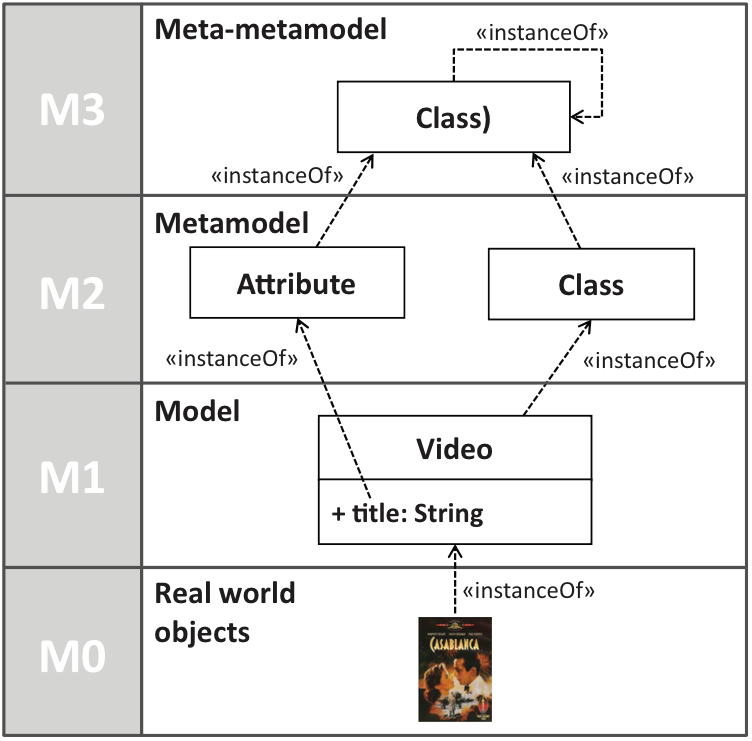
\includegraphics[scale=0.3]{images/models_notions}
\end{figure}

\begin{itemize}
	\item meta-metamodelo (M3): M3 constitui a base da arquitetura de meta-modelagem. A função primordial deste nível é definir linguagens para especificar meta-modelos. Um meta-metamodelo define um modelo de mais alto nível de abtração que o meta-modelo, e este primeiro é tipicamente mais compacto que o segundo. \sigla{MOF}{\emph{Meta-Object Facility}}~\cite{MOF} é \sigla{EMF}{\emph{Eclipse-Modeling Framework}}\cite{EMF} são exemplos de meta-metamodelos;
	\item meta-modelo (M2): um meta-modelo representa uma instância de um meta-metamodelo. A função principal do nível do meta-modelo é definir uma linguagem para especificar modelos. Os meta-modelos são tipicamentes mais elaborados que os meta-metamodelos. Por exemplo, a UML~\cite{UML:OMG} e o KDM~\cite{KDM:ISO} ambos possuem meta-modelos que os descrevem estruturalmente;
	\item modelo (M1): um modelo é uma instancia de um meta-modelo. A função principal do nível de modelo é definir uma linguagem para descrever um domínio específico;
	\item dados (M0): os objetos de usários representam os dados finais. A principal responsabilidade dos objetos de usuários é descrever um domínio específico em uma plataforma final.
\end{itemize}

% subsection modelos_e_meta_modelos (end)
\subsection{Transformação de Modelos}\label{sec:transformacoes_de_modelos}

A transformação em modelo desempenha um papel fundamental em abordagens que utilizam os princípios de MDE pois permite a manipulação de modelo de forma totalmente automática. Uma transformação consiste na geração automática de um modelo alvo tendo como base um modelo fonte, sendo que essa transformação foi definida por meio de um conjunto de regras de transformações~\cite{Mens_2006}. 

Nos trabalhos de~\citeonline{Mens_2006, Czarnecki_2006} e ~\citeonline{Biehl_2010} os autores buscam identificar e classificar as transformações de modelos. Algumas das classificações apresentadas por tais autores são citadas de forma resumida, a seguir:

\begin{itemize}
	\item Vertical ou Horizontal: Os modelos fonte e alvo podem estar em um ou mais níveis de abstração. Uma transformação horizontal mantêm modelos fonte e alvos no mesmo nível de abstração. Na transformação vertical, existe uma mudança de nível de abstração nos modelos. Esta mudança pode ser tanto para aumentar quanto par diminuir o nível de abstração;
	\item  Endógenas ou Exógenas: Nas transformações Endógeas os modelos envolvidos são expressos na mesma linguagem de modelagem. Nas transformações Exógenas os modelos que participam da transformação são de linguagens diferentes;
	\item Bidirecionais: Uma transformação bidirecional pode tanto gerar modelos alvos utilizando como base modelos fontes, quanto gerar modelos fontes utilizando modelos alvos. Em contrapartida, transformações unidirecionais, existe apenas uma fluxo de execução. 
\end{itemize}

As transformações do tipo classificadas como endógenas ou exógenas~\cite{Brambilla_2012} são apresentadas na Figura~\ref{fig:model_transformations}. Como pode ser observado na Figura~\ref{fig:model_transformations} transformações em modelos do tipo endógenas apenas um modelo e uma meta-modelo são utilizados, por outro lado, transformações do tipo exógenas os meta-modelos alvo e fonte são diferentes. Usualmente, refatorações em modelo são um exemplo de transformações do tipo endógenas, e uma transformação que tem como objetivo transformar uma linguagem para uma outra linguagem é um exemplo de transformações do tipo exógenas. Adicionalmente, é importante salientar que transformações em modelos que utilizam apenas um modelo como entrada e geram o mesmo modelo como saída com algumas modificações, essas transformações são classificadas como \aspas{\emph{in-place}}, enquanto que transformações em modelos que utilizam como entrada um modelo e tem como objetivo gerar um outro modelo como saída, tais transformações são consideradas \aspas{\emph{out-place}}. 

Transformações endógenas são mais interessantes quando apenas um subconjunto do modelo será afetado pela transformação~\cite{Brambilla_2012}. Por exemplo, em um editor de modelos transformações endógenas podem ser utilizadas para definir pequenas mudanças para automatizar tarefas repetitivas durante o desenvolvimento de modelos. Outra aplicação interessante de transformações endógenas é a condução de refatoração em nível de modelos. Um dos principais objetivos dessa tese de doutorado é a criação e utilização de refatoração em modelos, assim, maior enfase será concentrada em transformações de modelos do tipo endógenas no restante dessa subseção.

\begin{figure}[htb]
 \caption{Diferentes tipos de transformações em modelos: (a) \emph{exogenous} \aspas{\emph{out-place}} vs. (b) \emph{endogenous} \aspas{\emph{in-place}}}
 \label{fig:model_transformations}
 \centering
 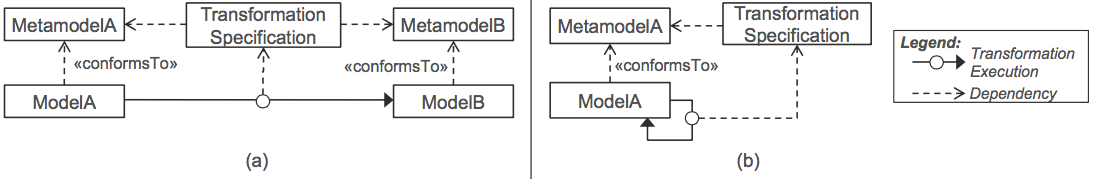
\includegraphics[scale=0.45]{images/transformacoes.png}
 \fadaptada{Brambilla_2012}
\end{figure}

Transformações endógenas usualmente são implementadas utilizando técnicas de \aspas{reescrita de grafo}, ou como também é conhecido \aspas{transformação de grafo}~\cite{Ehrig_2006}. Na teoria dos grafos, \aspas{reescrita de grafo} é um conjunto de regras para reescrever um determinado grafo, por exemplo, dado $p: \emph{left-hand side} (LHS) \rightarrow \emph{right-hand side} (RHS)$, sendo $LHS$ o grafo usado como padrão (no lado esquerdo) e $RHS$ o grafo de substituição (no lado direito da regra). Mais precisamente, o lado esquerdo, LHS, representa todas as pré-condições que devem ser satisfeitas antes da execução das regras de transformações. Similarmente, o lado direito, RHS, contêm todas as pós-condições. As ações que serão executadas pelas regras de transformações são implicitamente definidas tanto no grafo LHS quanto no grafo RHS. A execução de um conjunto de regra de transformação produz os seguintes efeitos: (\textit{i}) todos os elementos que apenas estão contidos no grafo LHS são deletados; (\textit{ii}) todos os elementos que apenas estão contidos no grafo RHS são adicionados; e (\textit{iii}) todos os elementos que estão contidos em ambos os grafos, LHS e RHS, são preservados~\cite{Ehrig_2006}. 

Neste contexto, \aspas{reescrita de grafo} é útil para auxiliar na definição de transformações de modelos e meta-modelos. Por exemplo, de acordo com~\citeonline{Lehnert_2012, Fluri_2006}, técnicas de \aspas{reescrita de grafo} podem ser aplicadas em qualquer meta-modelo e modelos que implementam o padrão MOF, ou seja, KDM, UML, entre outros. Qualquer instância de um meta-modelo que implemente o padrão MOF pode ser representado como um grafo da seguinte forma: (\textit{i}) vertices podem ser entendidos como: \texttt{EPackage}, \texttt{EClass}, \texttt{EDataType}, \texttt{EEnum}, \texttt{EAnotation}, \texttt{EOperation}, \texttt{EAttribute} e \texttt{EEnumLiteral}; (\textit{ii}) arestas pode ser representadas em meta-modelo como: \texttt{EReference}, \texttt{Inheritance}, \texttt{EAnnotationLink}. Assim, pode-se definir e realizar evoluções, simulações, refatorações de modelos por meio de técnicas de \aspas{reescrita de grafo}. 

% Dessa forma, as gramáticas de um grafo consistem de um conjunto de regras de transformações e um grafo inicial (geralmente referenciado como grafo \aspas{hospedeiro}) onde as regras de transformações são aplicadas. Usualmente as regras de transformações consistem de um grafo denominado \emph{left-hand side} (LHS) e um grafo \emph{right-hand side} (RHS). O grafo LHS tem como intuito representar todas as pré-condições para antes do conjunto de regras de transformações serem aplicadas no modelos. Similarmente, o grafo RHS contêm todas as pós-condições. As ações que serão executadas pelas regras de transformações são implicitamente definidas tanto no grafo LHS quanto no grafo RHS. Mais precisamente, a execução de um conjunto de regra de transformação produz os seguintes efeitos: (\textit{i}) todos os elementos que apenas estão contidos no grafo LHS são deletados; (\textit{ii}) todos os elementos que apenas estão contidos no grafo RHS são adicionados; e (\textit{iii}) todos os elementos que estão contidos em ambos os grafos, LHS e RHS, são preservados. 

Comumente, transformações em modelos são desenvolvidas utilizando linguagens especializadas, denominadas de linguagens de transformação de modelos. Diversas linguagens de transformação de modelos têm sido propostas atualmente~\cite{Allilaire_06, Biehl_2010}. Cada linguagem tipicamente fornece um conjunto de características que a torna mais apropriada para o tipo de transformação almejada. No trabalho de~\citeonline{Biehl_2010}, são citadas várias linguagens de transformação de modelos, o que mostra uma dimensão do número de linguagens para transformação de modelos existentes e disponíveis para o usuário atualmente. Algumas das linguagens citadas são: ATL~\cite{ATL_eclipse,Jouault_2008}, \sigla{QVT}{\textit{Query/View/Transformation}}~\cite{QVT:OMG}, EMF Henshin~\cite{EMF_Henshin}, SmartQVT~\cite{SmartQVT}, ModelMorf~\cite{ModelMorf}, Kermeta~\cite{kermeta}, \sigla{ETL}{\textit{Epsilon Transformation Language}}~\cite{ETL_eclipse}, \sigla{OAW}{OpenArchitectureWare}~\cite{OpenArchitectureWare}, VIATRA~\cite{viatra}, AndroMDA~\cite{andromda} e Fujaba transformations~\cite{fujaba}.

Nos trabalhos~\cite{Biehl_2010, Mens_2006, Allilaire_06}, os autores buscam levantar caracteristicas importantes tanto para classificar as transformações de modelos, quanto as linguagens de transformação de modelos  para realizaçnao destas transformações. Similarmente,~\citeonline{transformation_huber} busca avaliar diferentes ferramentas e linguagens de transformação de modelos. O estudo conclui que nenhuma ferramenta é melhor do que a outra, mas que uma linguagem pode ser mais adequada para um problema específico do que outras linguagens. Entre as várias características utilizadas pelos autores na classificação das linguagens de transformação, a característica de maior importância é quanto ao paradigma da linguagem. Segundo~\citeonline{Mens_2006}, a maior distinção entre os mecanismo de transformação de modelos é quanto ao seu paradigma. Os principais paradigmas das linguagens de transformações de modelos, são descritos, a seguir:

\begin{itemize}
	\item Imperativo: Linguagens imperativas especificam um fluxo de controle sequencial e fornecem meios para descrever a forma como a linguagem de transformação de modelo supostamente deve ser executada~\cite{Mens_2006}. As construções e conceitos de linguagens de transformações imperativas são semelhantes as linguagens de programação de propósito geral, como Java ou C;
	\item Declarativo: Linguagens declarativas não oferecem um fluxo de controle explícito. Em vez de como a transformação deve ser executada, o foco é sobre o que deve ser mapeado pela transformação~\cite{Mens_2006}. Transformações de modelos declarativas descrevem a relação entre os meta-modelos fonte e alvo, onde esta relação pode ser interpretada bidirecionalmente. Em geral, tais linguagens são compactas e as descrições de transformações são geralmente curtas e concisas~\cite{Biehl_2010, Mens_2006};
	\item Híbrido: Linguagens de transformação híbridas oferecem tanto as construções de linguagem imperativa quanto as construções de linguagem declarativa;
	\item Transformação Direta: Linguagens de programação de uso geral e bibliotecas para ler e gravar os dados dos modelos são utilizadas para implementar as transformações de modelos~\cite{transformation_huber}. A vantagem da transformação direta é que os programadores não precisam aprender uma nova linguagem. Mas por outro lado, as implementações tendem a se tornar maiores~\cite{Biehl_2010}.
\end{itemize}


%Na literatura é possível identificar um conjunto de linguagens especificadas para auxiliar a realização de transformações em modelos. Por exemplo, VIATRA [16], AGG [17], Henshin [18], ATOM [19], ETL, ATL, QVT. De acordo com Livro MDD ATL é a linguagem de transformações em modelos mais utilizada tanto academicamente quanto industrialmente. Dessa forma, nesta tese de doutorado optou-se por utilizar a ATL para a definição de transformações em modelos. Na subseção a seguir é apresentado como a ATL pode ser utilizada para a realização de transformações em modelos.

\subsection{ATLAS \emph{Transformation Language} (ATL)} % (fold)
\label{sub:atl_transformation_language}

A ATLAS \emph{Transformation Language} (ATL)~\cite{ATL_eclipse} é uma linguagem de transformação de modelo híbrida, ou seja, a linguagem contêm uma mistura de construções declarativas e imperativas. O uso do estilo declarativo é encorajado por vários autores~\cite{Allilaire_06, Jouault_2005, Jouault_2008}, pois permite uma implementação mais objetiva e mais simples. No entanto, a definição de transformações complexas utilizando apenas construções declarativas pode ser uma tarefa difícil. Nesse caso, os desenvolvedores podem recorrer aos recursos imperativos da linguagem~\cite{Allilaire_06}.

A ATL possui uma sintaxe abstrata definida utilizando um meta-modelo. Isso significa que cada transformação definida em ATL é de fato um modelo. Uma transformação ATL pode ser decomposta em três partes: um \textit{header}, \textit{helpers} e um conjunto de \textit{rules}. O \textit{header} (cabeçalho) é utilizado para declarar informações gerais, tais como o nome do módulo (nome da transformação que deve coincidir com o nome do arquivo .atl), os meta-modelos de entrada e de saída  e a importação de bibliotecas necessárias. Os \textit{helpers} são sub-rotinas que são usados para evitar a redundância de código. Pode-se imaginar um \textit{helper} como um método igual tem-se em linguagens de programação. Já as \textit{rules} (regras) são as principais definições das transformações ATL, porque elas descrevem como os elementos de saída (em conformidade com o meta-modelo de saída) são produzidos a partir de elementos de entrada (em conformidade com o meta-modelo de entrada). Elas são constituídas por ligações, cada uma expressando um mapeamento entre um elemento de entrada e um elemento de saída~\cite{ATL_eclipse}.

O funcionamento da ATL se dá da seguinte forma. Primeiro o código ATL deve ser compilado e, em seguida, executado pelo mecanismo de transformação ATL. A ATL oferece suporte dedicado para rastreabilidade. A ordem de execução das regras é determinada automaticamente, com exceção das \textit{Lazy Rules}, que precisam ser chamadas explicitamente no código da ATL. Os \textit{helpers} fornecem construções imperativas às transformações. A ATL também contêm um modulo denominada ATL Refining que suporta transformações do tipo \emph{endogenous} \aspas{\emph{in-place}}.

A ATL foi escolhida para implementação deste trabalho considerando vários aspectos. A ATL está integrada na plataforma Eclipse, o que provê uma série de recursos padrões para desenvolveimento (\textit{syntax highlighting} e \textit{debugger}). A ATL é parte do projeto \sigla{M2M}{Model-To-Model} da ferramenta Eclipse e possui um grupo de discussão ativo, constatemente atualizado, vários exemplos e diversos estudos de casos aplicados até mesmo na indústria\footnote{\texttt{https://www.eclipse.org/forums/index.php?t=thread&frm_id=241}} utilizam a ATL. Por se tratar de uma ferramenta de fácil uso, a partir de premissa de conhecimento de linguagem e do meta-modelo, traz como vantagem ao processo: baixo custo, por ser uma ferramenta livre, e alta flexibilidade, por facilitar grandes alterações na transformação diretamente usando a interface do editor de regras ATL~\cite{Salem_2008}. Além disso, a ATL é uma das linguagens de transformações mais madura no contexto da MDE~\cite{bruneliere_2010}.

\section{Refatoração}\label{sec:refatoracao}


Refatoração pode ser entendido como um processo de redistribuição de funcionalidade com o intuito de melhorar um dado sistema. No contexto do paradigma orientado a objeto, essa redistribuição está totalmente ligada com classes, atributos e operações. Isto é, a refatoração tem como objetivo permitir a redistribuição de classes, atributos e operações na hierarquia de classes para facilitar futuras atividades de desenvolvimento ou de manutenção. A primeira definição de refatoração foi concebida por~\citeonline{OPDYKE_1992} em sua tese da seguinte forma: \aspas{refatorações são transformações que reestruturam um determinado sistema com o objetivo de melhorar o \textit{design}, evolução e reuso de sistemas desenvolvidos no paradigma orientada a objeto}.

No contexto do paradigma orientado a objeto, refatoração é uma alternativa do conceito de reestruturação. Em outras palavras, refatoração é um termo aplicado ao paradigma orientado a objeto; para outros paradigmas de programação, esse mesmo processo é descrito como reestruturação~\cite{Chikofsky_cross}. De acordo com~\citeonline{Chikofsky_cross}, reestruturação \aspas{consiste no processo de alterar um software, melhorando a sua estrutura interna, de forma que o comportamento externo do código não seja alterado}. Reestruturação e refatoração são técnicas essenciais que são utilizadas para mitigar problemas relacionados à evolução de software~\cite{OPDYKE_1992}. Com o objetivo de aumentar atributos de qualidade dos sistemas, as práticas de refatoração surgiram através do emprego de reestruturação sobre unidades de código preservando o seu comportamento~\cite{Chikofsky_cross,OPDYKE_1992}.

Quando aplicada durante a fase de manutenção de software, a refatoração ajuda a tornar o código mais legível e também tem como objetivo solucionar problemas de códigos mal escritos~\cite{Chikofsky_cross}. A refatoração também pode ser usada no contexto da reengenharia, ou seja, para alterar um sistema específico visando reconstruí-lo em um novo formato. Nesse contexto, a refatoração é necessária para converter código legado ou deteriorado em um formato mais estruturado ou modular, ou para migrar o código para uma diferente linguagem de programação, ou mesmo um diferente paradigma de linguagem.

Em seu livro,~\citeonline{Fowler1999}, apresenta duas definições para refatoração, uma como substantivo e outra como verbo:

\begin{itemize}
	\item Refatoração: uma mudança que é realizada na estrutura interna de um determinado sistema com o objetivo de deixar o sitema mais fácil de entender e fácil de modificar sem alterar o seu comportamento externo; e
	\item Refatorar: reestruturar o software por meio de um conjunto de refatorações sem modificar o seu comportamento externo.
\end{itemize}

As definições apresentadas por~\citeonline{Fowler1999} enfatizam que o propósito da refatoração é fazer com que o software fique mais fácil de entender (melhorar sua compreensão) e de modificar (melhorar sua manutenibilidade). Outra caractetistica de suma importância a ser destacada é que a refatorações em geral deve ser um processo para melhorar o \textit{design} do software. De acordo com~\citeonline{Wake_2003} , refatoração é \aspas{uma arte para melhorar cuidadosamente o \textit{design} de códigos existentes.} O autor também enfatiza que refatoração deve fornecer maneiras de identificar problemas no código e também deve prover soluções para corrigir tais problemas.~\citeonline{Wake_2003} caracteriza refatoração como:

\begin{itemize}
	\item refatoração não inclui nenhuma mudança no sistema - refatoração não devê adicionar novas funcionalidades ao sistema;
	\item refatoração deve ser utilizada para melhorar o código do sistema;
	\item nem toda reestruturação pode ser considerada como refatoração - usualmente refatorações tendem a serem transformações pequenas e seguras. 
\end{itemize}

O primeiro conjunto de refatorações foi proposto por~\citeonline{OPDYKE_1992}, onde o autor defini 26 refactorações de baixa granularidade. Tais refatorações podem ser resumidas da seguinte forma:

\begin{itemize}
	\item criar um membro  - variável/função/classe: Essas refatorações tem como objetivo criar novas variáveis e/ou funções para uma classe em particular ou criar um nova classe;
	\item deletar um membro - variável/função/classe. Essas refatorações tem como objetivo  deletar membros que não estão sendo utilizados;
	\item renomear um membro - variável/função/classe. Essas refatorações podem ser utilizadas pare renomear membros e fornecerem nomes mais significativos;
	\item mover um membro - variável/função. Essas refatorações são utilizadas para redistribuir um conjunto de variáveis/funções para sub ou super-classes.
\end{itemize}

Similarmente,~\citeonline{Roberts_1999} defini um conjunto de refatorações que devem ser aplicadas em classes, métodos e atríbutos. Porém o catálogo mais completo e extensivo de refatorações foi definido por~\citeonline{Fowler1999}. Neste catalogo cada refatoração possui os seguintes tópicos: (\textit{i}) um nome, (\textit{ii}) uma breve descrição, (\textit{iii}) uma motivação para a condução da refatoração, (\textit{iv}) um mecanismo descrevendo como a refatoração deve ser executada e (\textit{v}) um exemplo ilustrando a utilização da refatoração. As refatorações proposta por~\citeonline{Fowler1999} são agrupadas em setes categorias, a saber: (\textit{i}) \textit{Composing Methods}, (\textit{ii}) \textit{Moving Features Between Objects}, (\textit{iii}) \textit{Organizing Data}, (\textit{iv}) \textit{Simplifying Conditional Expressions}, (\textit{v}) \textit{Make Method Calls Simpler}, (\textit{vi}) \textit{Dealing with Generalization} e (\textit{vii}) \textit{Big Refactorings}.

De acordo com~\citeonline{Fowler1999} existem quatro principais motivações para a aplicação de refatoração:

\begin{enumerate}
	\item refatorações quando bem conduzidas tendem a melhorar o \textit{design} do software - dessa forma, refatoração pode auxiliar na prevenção da decadência do software e eliminando código duplicado;
	\item refatorações fazem com que o código-fonte fique mais fácil de entender - código bem legível facilita a comunicação e seu propósito;
	\item refatoração auxilia na identificação de erros - melhorando a estrutura interna do código-fonte erros tendem a serem identificados mais facilmente;
	\item desenvolvimento mais produtivo - uma boa estrutura interna usualmente facilita o desenvolvimento e melhora a produtividade.
\end{enumerate}

Como já salientado refatorações devem preservar o comportamento de um determinado software após a aplicação de \textit{n} refatorações. Dessa forma,~\citeonline{Mens_and_Tourwe_2004,Cinneide_2000} relatam que existem três principais abordagens para auxiliar a preservação (de alguns aspectos) do comportamento do código-fonte. Tais abordagens são: (\textit{i}) abordagem não formal (por exemplo, as refatorações definidas por~\citeonline{Fowler1999}), (\textit{ii}) uma abordagem semi-formal~\cite{Roberts_1999} e (\textit{iii}) abordagem completamente formal. No entanto, os autores também argumentam que mesmo com a utilização da última abordagem é impossível garantir totalmente a preservação de comportamento ápos a aplicação de refatorações~\cite{Mens_and_Tourwe_2004,Cinneide_2000}.% A ideia de preservação de comportamento no contexto de refatoração foi primeiramente introduzida por~\citeonline{OPDYKE_1992} da seguinte forma: \aspas{se um programa é chamado duas vezes (antes e depois da refatoração) com o mesmo conjunto de entradas, o resultado deve ser o mesmo}  


Usualmente o processo para a aplicação de um refatoração contêm três principais passos~\cite{Wake_2003}. O primeiro passo consiste na identificação de partes do código que precisam ser refatoradas. O segundo passo consiste na escolha do melhor refatoração para solucionar o problema anteriormente identificado. O terceiro passo consiste na aplicação da refatoração.

\section{Considerações Finais}

Neste capítulo foi apresentada uma revisão dos principais conceitos envolvendo reengenharia de software, engenharia dirigido por modelos e refatoração que são relevantes para a proposta desta tese. Foram apresentados os principais termos relacionados a reengenharia de software. Além disso, também foram discutidos e apresentados todas as etapas que devem ser realizadas para a condução da engenharia dirigida por modelos, ou seja, todos os níveis CIM, PIM e PSM foram apresentados. Em seguida, foi apresentado a definição e diferença de meta-metamodelo, metamodelo, modelo e dados. Posteriormente, transformações em modelos foram apresentadas e discutidas, salientado as principais classificação transformações encontradas na literatura - vertical ou horizontal, endógenas ou exógenas. Ainda em relação a transformação de modelos, algumas das principais linguagens utilizadas para realizar a transformação em modelos também foram apresentadas. Porém, apenas a linguagem ATL foi discutida com maiores informações. Os conceitos sobre refatoração também foram apresentados.

No próximo capítulo são apresentados os principais conceitos envolvendo Modernização Orientada à Arquitetura e KDM.